\clearpage
\subsection{MSVC + \olly}
\index{\olly}

\RU{Загрузим наш пример в \olly и установим точку останова на функции \comp}
\EN{Let's load our example into \olly and set a breakpoint on \comp}.

\RU{Как значения сравниваются, мы можем увидеть во время самого первого вызова \comp}
\EN{We can see how the values are compared at the first \comp call}:

\begin{figure}[H]
\centering
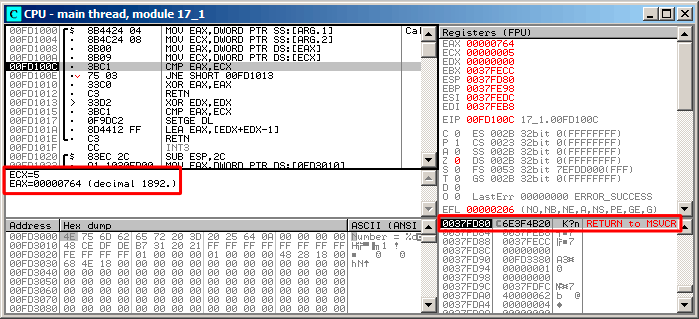
\includegraphics[scale=\FigScale]{patterns/18_pointers_to_functions/olly1.png}
\caption{\olly: \RU{первый вызов}\EN{first call of} \comp}
\label{fig:qsort_olly1}
\end{figure}

\RU{Для удобства, }\olly \RU{показывает сравниваемые значения в окне под окном кода}
\EN{shows the compared values in the window under the code window, for convenience}.
\RU{Мы можем так же увидеть, что}\EN{We can also see that the} \ac{SP} \RU{указывает на}\EN{points to} 
\ac{RA} \RU{где находится место в функции}\EN{, where the} 
\qsort \EN{function is }(\RU{на самом деле, находится в}\EN{located in} \TT{MSVCR100.DLL}).

\clearpage
\RU{Трассируя}\EN{By tracing} (F8) \RU{до инструкции}\EN{until the} \TT{RETN} 
\RU{и нажав F8 еще один раз, мы возвращаемся в функцию}\EN{instruction and pressing F8 one more time, 
we return to the} \qsort\EN{ function}:

\begin{figure}[H]
\centering
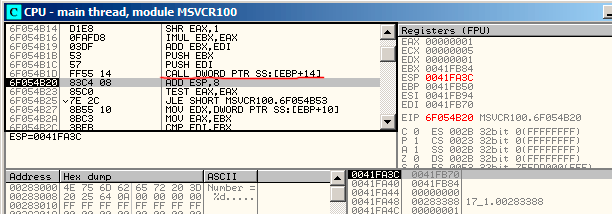
\includegraphics[scale=\FigScale]{patterns/18_pointers_to_functions/olly2.png}
\caption{\olly: \RU{код в}\EN{the code in} \qsort \RU{сразу после вызова}\EN{right after} \comp\EN{ call}}
\label{fig:qsort_olly2}
\end{figure}

\RU{Это был вызов функции сравнения}\EN{That was a call to the comparison function}.

\clearpage
\RU{Вот также скриншот момента второго вызова функции}\EN{Here is also a screenshot of the moment of the 
second call of} \comp\EMDASH{}\RU{теперь сравниваемые значения другие}
\EN{now values that have to be compared are different}:

\begin{figure}[H]
\centering
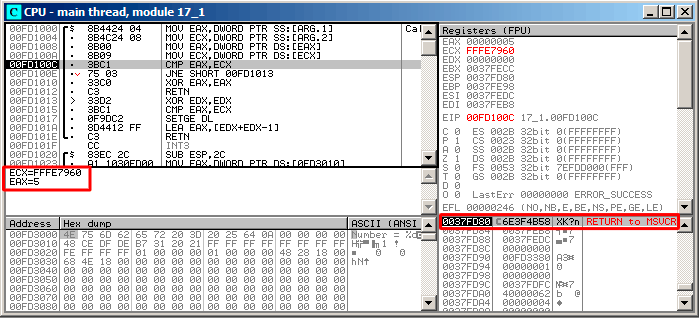
\includegraphics[scale=\FigScale]{patterns/18_pointers_to_functions/olly3.png}
\caption{\olly: \RU{второй вызов}\EN{second call of} \comp}
\label{fig:qsort_olly3}
\end{figure}
